\documentclass[14pt]{extbook}
\usepackage{multicol, enumerate, enumitem, hyperref, color, soul, setspace, parskip, fancyhdr} %General Packages
\usepackage{amssymb, amsthm, amsmath, latexsym, units, mathtools} %Math Packages
\everymath{\displaystyle} %All math in Display Style
% Packages with additional options
\usepackage[headsep=0.5cm,headheight=12pt, left=1 in,right= 1 in,top= 1 in,bottom= 1 in]{geometry}
\usepackage[usenames,dvipsnames]{xcolor}
\usepackage{dashrule}  % Package to use the command below to create lines between items
\newcommand{\litem}[1]{\item#1\hspace*{-1cm}\rule{\textwidth}{0.4pt}}
\pagestyle{fancy}
\lhead{Progress Quiz 9}
\chead{}
\rhead{Version ALL}
\lfoot{9541-5764}
\cfoot{}
\rfoot{Summer C 2021}
\begin{document}

\begin{enumerate}
\litem{
First, find the equation of the line containing the two points below. Then, write the equation in the form $ y=mx+b $ and choose the intervals that contain $m$ and $b$.\[ (4, -10) \text{ and } (-10, 4) \]\begin{enumerate}[label=\Alph*.]
\item \( m \in [-3.2, -0.3] \hspace*{3mm} b \in [4, 12] \)
\item \( m \in [-3.2, -0.3] \hspace*{3mm} b \in [-12, -3] \)
\item \( m \in [0.8, 1.1] \hspace*{3mm} b \in [10, 18] \)
\item \( m \in [-3.2, -0.3] \hspace*{3mm} b \in [10, 18] \)
\item \( m \in [-3.2, -0.3] \hspace*{3mm} b \in [-15, -11] \)

\end{enumerate} }
\litem{
Solve the equation below. Then, choose the interval that contains the solution.\[ -16(-11x + 2) = -5(17x -18) \]\begin{enumerate}[label=\Alph*.]
\item \( x \in [-0.38, -0.21] \)
\item \( x \in [0.46, 0.71] \)
\item \( x \in [-1.16, -0.56] \)
\item \( x \in [-0.07, 0.29] \)
\item \( \text{There are no real solutions.} \)

\end{enumerate} }
\litem{
Solve the equation below. Then, choose the interval that contains the solution.\[ -9(3x -19) = -12(7x -18) \]\begin{enumerate}[label=\Alph*.]
\item \( x \in [0.4, 0.9] \)
\item \( x \in [4.7, 7] \)
\item \( x \in [-8.5, -6.5] \)
\item \( x \in [2.8, 3.8] \)
\item \( \text{There are no real solutions.} \)

\end{enumerate} }
\litem{
First, find the equation of the line containing the two points below. Then, write the equation in the form $ y=mx+b $ and choose the intervals that contain $m$ and $b$.\[ (-8, 11) \text{ and } (-3, -8) \]\begin{enumerate}[label=\Alph*.]
\item \( m \in [3.8, 4.8] \hspace*{3mm} b \in [3.27, 3.59] \)
\item \( m \in [-11.8, -1.8] \hspace*{3mm} b \in [19.25, 19.6] \)
\item \( m \in [-11.8, -1.8] \hspace*{3mm} b \in [-5.52, -4.94] \)
\item \( m \in [-11.8, -1.8] \hspace*{3mm} b \in [18.55, 19.3] \)
\item \( m \in [-11.8, -1.8] \hspace*{3mm} b \in [-19.71, -19.2] \)

\end{enumerate} }
\litem{
Find the equation of the line described below. Write the linear equation in the form $ y=mx+b $ and choose the intervals that contain $m$ and $b$.\[ \text{Perpendicular to } 8 x + 7 y = 6 \text{ and passing through the point } (4, 5). \]\begin{enumerate}[label=\Alph*.]
\item \( m \in [0.83, 1] \hspace*{3mm} b \in [1.41, 2.39] \)
\item \( m \in [-0.9, -0.74] \hspace*{3mm} b \in [8.16, 8.58] \)
\item \( m \in [0.83, 1] \hspace*{3mm} b \in [-1.77, -1.45] \)
\item \( m \in [0.83, 1] \hspace*{3mm} b \in [0.58, 1.29] \)
\item \( m \in [0.98, 1.25] \hspace*{3mm} b \in [1.41, 2.39] \)

\end{enumerate} }
\litem{
Write the equation of the line in the graph below in Standard Form $Ax+By=C$. Then, choose the intervals that contain $A, B, \text{ and } C$.
\begin{center}
    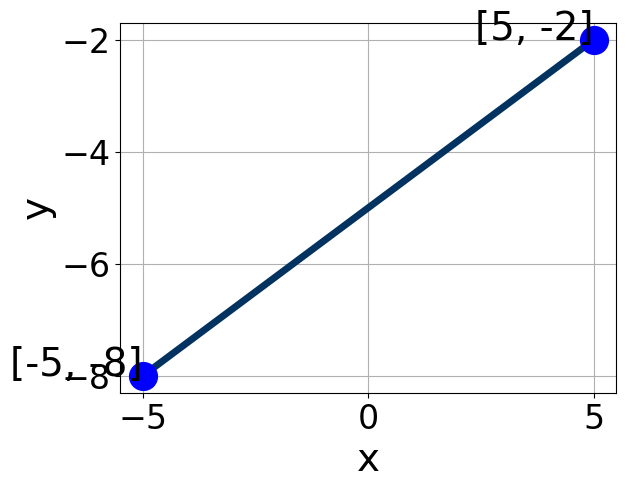
\includegraphics[width=0.5\textwidth]{../Figures/linearGraphToStandardA.png}
\end{center}
\begin{enumerate}[label=\Alph*.]
\item \( A \in [-2.7, 1.1], \hspace{3mm} B \in [-4.6, 0.3], \text{ and } \hspace{3mm} C \in [1, 7] \)
\item \( A \in [2.5, 5], \hspace{3mm} B \in [3.8, 5.1], \text{ and } \hspace{3mm} C \in [-31, -22] \)
\item \( A \in [2.5, 5], \hspace{3mm} B \in [-6, -1.5], \text{ and } \hspace{3mm} C \in [23, 28] \)
\item \( A \in [-4.8, -2.7], \hspace{3mm} B \in [3.8, 5.1], \text{ and } \hspace{3mm} C \in [-31, -22] \)
\item \( A \in [-2.7, 1.1], \hspace{3mm} B \in [0.9, 2.6], \text{ and } \hspace{3mm} C \in [-7, -4] \)

\end{enumerate} }
\litem{
Solve the linear equation below. Then, choose the interval that contains the solution.\[ \frac{3x + 6}{8} - \frac{-3x -8}{5} = \frac{9x + 5}{7} \]\begin{enumerate}[label=\Alph*.]
\item \( x \in [27.97, 30.97] \)
\item \( x \in [5.26, 6.26] \)
\item \( x \in [-0.45, 1.55] \)
\item \( x \in [-8.03, -4.03] \)
\item \( \text{There are no real solutions.} \)

\end{enumerate} }
\litem{
Solve the linear equation below. Then, choose the interval that contains the solution.\[ \frac{4x + 9}{3} - \frac{-9x + 3}{7} = \frac{5x -4}{2} \]\begin{enumerate}[label=\Alph*.]
\item \( x \in [-5.57, 0.43] \)
\item \( x \in [-84, -80] \)
\item \( x \in [-41.4, -36.4] \)
\item \( x \in [-45.6, -43.6] \)
\item \( \text{There are no real solutions.} \)

\end{enumerate} }
\litem{
Write the equation of the line in the graph below in Standard Form $Ax+By=C$. Then, choose the intervals that contain $A, B, \text{ and } C$.
\begin{center}
    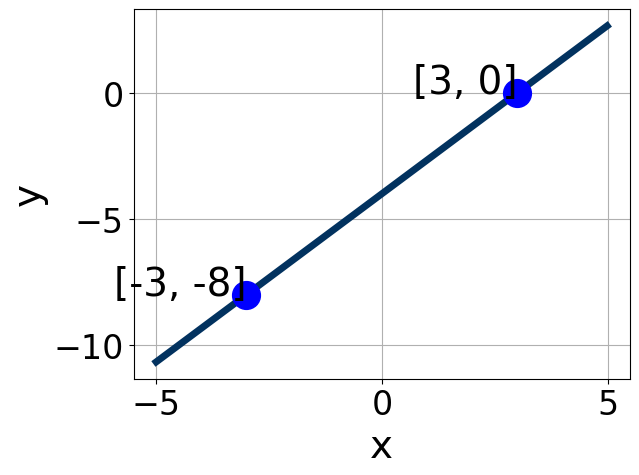
\includegraphics[width=0.5\textwidth]{../Figures/linearGraphToStandardCopyA.png}
\end{center}
\begin{enumerate}[label=\Alph*.]
\item \( A \in [-2.2, 0.8], \hspace{3mm} B \in [-0.09, 1.58], \text{ and } \hspace{3mm} C \in [-7, -3] \)
\item \( A \in [-4.6, -2.6], \hspace{3mm} B \in [1.71, 3.62], \text{ and } \hspace{3mm} C \in [-13, -10] \)
\item \( A \in [1.9, 4.6], \hspace{3mm} B \in [-3.18, -2.15], \text{ and } \hspace{3mm} C \in [12, 16] \)
\item \( A \in [-2.2, 0.8], \hspace{3mm} B \in [-1.34, -0.92], \text{ and } \hspace{3mm} C \in [0, 9] \)
\item \( A \in [1.9, 4.6], \hspace{3mm} B \in [1.71, 3.62], \text{ and } \hspace{3mm} C \in [-13, -10] \)

\end{enumerate} }
\litem{
Find the equation of the line described below. Write the linear equation in the form $ y=mx+b $ and choose the intervals that contain $m$ and $b$.\[ \text{Perpendicular to } 3 x + 8 y = 4 \text{ and passing through the point } (4, -10). \]\begin{enumerate}[label=\Alph*.]
\item \( m \in [2.5, 4.8] \hspace*{3mm} b \in [-16, -9] \)
\item \( m \in [2.5, 4.8] \hspace*{3mm} b \in [-23.67, -19.67] \)
\item \( m \in [-0.5, 2.6] \hspace*{3mm} b \in [-23.67, -19.67] \)
\item \( m \in [2.5, 4.8] \hspace*{3mm} b \in [17.67, 22.67] \)
\item \( m \in [-5.3, -1.6] \hspace*{3mm} b \in [-1.33, 3.67] \)

\end{enumerate} }
\litem{
First, find the equation of the line containing the two points below. Then, write the equation in the form $ y=mx+b $ and choose the intervals that contain $m$ and $b$.\[ (10, 9) \text{ and } (2, -4) \]\begin{enumerate}[label=\Alph*.]
\item \( m \in [1.62, 7.62] \hspace*{3mm} b \in [-7.32, -6.9] \)
\item \( m \in [1.62, 7.62] \hspace*{3mm} b \in [-6.14, -5.46] \)
\item \( m \in [1.62, 7.62] \hspace*{3mm} b \in [6.74, 7.29] \)
\item \( m \in [-4.62, -0.62] \hspace*{3mm} b \in [-0.91, 0.3] \)
\item \( m \in [1.62, 7.62] \hspace*{3mm} b \in [-1.54, -0.91] \)

\end{enumerate} }
\litem{
Solve the equation below. Then, choose the interval that contains the solution.\[ -11(15x + 4) = -7(2x + 18) \]\begin{enumerate}[label=\Alph*.]
\item \( x \in [1.1, 1.29] \)
\item \( x \in [-0.99, -0.75] \)
\item \( x \in [-1.81, -1.09] \)
\item \( x \in [0.54, 0.79] \)
\item \( \text{There are no real solutions.} \)

\end{enumerate} }
\litem{
Solve the equation below. Then, choose the interval that contains the solution.\[ -8(-9x -19) = -16(2x + 11) \]\begin{enumerate}[label=\Alph*.]
\item \( x \in [-0.37, 0.13] \)
\item \( x \in [0.17, 0.39] \)
\item \( x \in [0.53, 1.1] \)
\item \( x \in [-3.47, -3.09] \)
\item \( \text{There are no real solutions.} \)

\end{enumerate} }
\litem{
First, find the equation of the line containing the two points below. Then, write the equation in the form $ y=mx+b $ and choose the intervals that contain $m$ and $b$.\[ (7, -3) \text{ and } (-8, -11) \]\begin{enumerate}[label=\Alph*.]
\item \( m \in [-0.94, 0.53] \hspace*{3mm} b \in [-17.27, -11.27] \)
\item \( m \in [0.52, 0.71] \hspace*{3mm} b \in [-13, -8] \)
\item \( m \in [0.52, 0.71] \hspace*{3mm} b \in [-5, 3] \)
\item \( m \in [0.52, 0.71] \hspace*{3mm} b \in [2.73, 8.73] \)
\item \( m \in [0.52, 0.71] \hspace*{3mm} b \in [-7.73, -3.73] \)

\end{enumerate} }
\litem{
Find the equation of the line described below. Write the linear equation in the form $ y=mx+b $ and choose the intervals that contain $m$ and $b$.\[ \text{Parallel to } 4 x + 9 y = 11 \text{ and passing through the point } (-2, -8). \]\begin{enumerate}[label=\Alph*.]
\item \( m \in [-0.68, -0.35] \hspace*{3mm} b \in [8.15, 10.53] \)
\item \( m \in [-2.63, -2.21] \hspace*{3mm} b \in [-9.38, -8.49] \)
\item \( m \in [-0.68, -0.35] \hspace*{3mm} b \in [-6.29, -5.34] \)
\item \( m \in [-0.68, -0.35] \hspace*{3mm} b \in [-9.38, -8.49] \)
\item \( m \in [0.21, 1.07] \hspace*{3mm} b \in [-7.77, -6.24] \)

\end{enumerate} }
\litem{
Write the equation of the line in the graph below in Standard Form $Ax+By=C$. Then, choose the intervals that contain $A, B, \text{ and } C$.
\begin{center}
    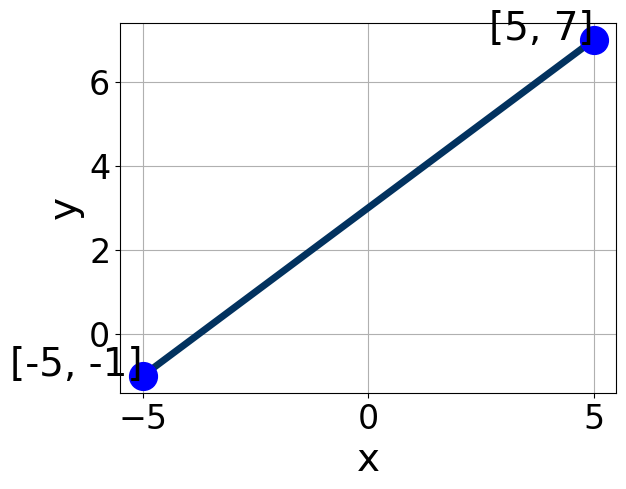
\includegraphics[width=0.5\textwidth]{../Figures/linearGraphToStandardB.png}
\end{center}
\begin{enumerate}[label=\Alph*.]
\item \( A \in [-3.1, 0.9], \hspace{3mm} B \in [-3, -0.4], \text{ and } \hspace{3mm} C \in [-8, -1] \)
\item \( A \in [-7.1, -2.2], \hspace{3mm} B \in [4.9, 6.3], \text{ and } \hspace{3mm} C \in [10, 18] \)
\item \( A \in [0.7, 7.4], \hspace{3mm} B \in [-7.4, -2.9], \text{ and } \hspace{3mm} C \in [-18, -13] \)
\item \( A \in [-3.1, 0.9], \hspace{3mm} B \in [0.1, 2.7], \text{ and } \hspace{3mm} C \in [-1, 4] \)
\item \( A \in [0.7, 7.4], \hspace{3mm} B \in [4.9, 6.3], \text{ and } \hspace{3mm} C \in [10, 18] \)

\end{enumerate} }
\litem{
Solve the linear equation below. Then, choose the interval that contains the solution.\[ \frac{5x + 6}{2} - \frac{7x + 4}{3} = \frac{-4x -4}{7} \]\begin{enumerate}[label=\Alph*.]
\item \( x \in [-7.26, -6.33] \)
\item \( x \in [-3.47, -2.8] \)
\item \( x \in [-1.27, -0.3] \)
\item \( x \in [-8.52, -7.79] \)
\item \( \text{There are no real solutions.} \)

\end{enumerate} }
\litem{
Solve the linear equation below. Then, choose the interval that contains the solution.\[ \frac{-7x + 8}{2} - \frac{-5x -7}{8} = \frac{-6x + 3}{5} \]\begin{enumerate}[label=\Alph*.]
\item \( x \in [-2.9, -0.5] \)
\item \( x \in [6.7, 7.5] \)
\item \( x \in [1.2, 1.8] \)
\item \( x \in [2.4, 3] \)
\item \( \text{There are no real solutions.} \)

\end{enumerate} }
\litem{
Write the equation of the line in the graph below in Standard Form $Ax+By=C$. Then, choose the intervals that contain $A, B, \text{ and } C$.
\begin{center}
    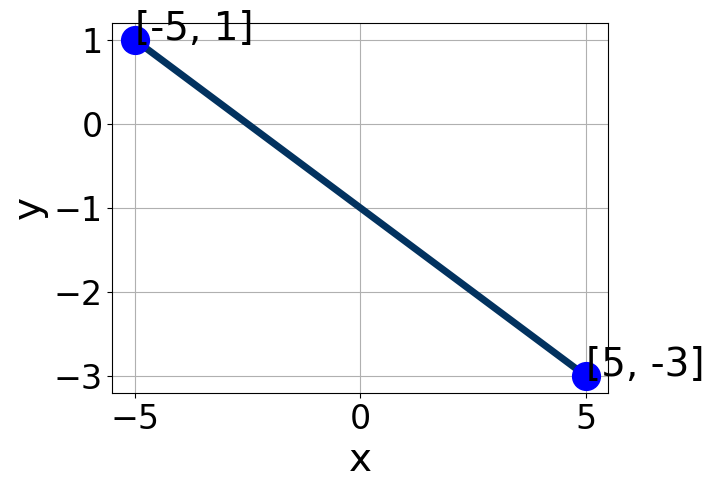
\includegraphics[width=0.5\textwidth]{../Figures/linearGraphToStandardCopyB.png}
\end{center}
\begin{enumerate}[label=\Alph*.]
\item \( A \in [-2.53, -1.94], \hspace{3mm} B \in [-5.7, -3.7], \text{ and } \hspace{3mm} C \in [4.46, 6.57] \)
\item \( A \in [-0.18, 1.68], \hspace{3mm} B \in [-0.5, 2.4], \text{ and } \hspace{3mm} C \in [-2.19, -0.77] \)
\item \( A \in [-0.18, 1.68], \hspace{3mm} B \in [-3.2, -0.3], \text{ and } \hspace{3mm} C \in [0.79, 1.05] \)
\item \( A \in [1.39, 2.92], \hspace{3mm} B \in [-5.7, -3.7], \text{ and } \hspace{3mm} C \in [4.46, 6.57] \)
\item \( A \in [1.39, 2.92], \hspace{3mm} B \in [4.8, 5.4], \text{ and } \hspace{3mm} C \in [-5.32, -3.7] \)

\end{enumerate} }
\litem{
Find the equation of the line described below. Write the linear equation in the form $ y=mx+b $ and choose the intervals that contain $m$ and $b$.\[ \text{Parallel to } 3 x + 7 y = 8 \text{ and passing through the point } (-5, 7). \]\begin{enumerate}[label=\Alph*.]
\item \( m \in [-0.99, 0.22] \hspace*{3mm} b \in [-4.86, -1.86] \)
\item \( m \in [-0.99, 0.22] \hspace*{3mm} b \in [-0.14, 5.86] \)
\item \( m \in [-3.3, -1.72] \hspace*{3mm} b \in [-0.14, 5.86] \)
\item \( m \in [-0.99, 0.22] \hspace*{3mm} b \in [12, 16] \)
\item \( m \in [-0.39, 0.98] \hspace*{3mm} b \in [9.14, 10.14] \)

\end{enumerate} }
\litem{
First, find the equation of the line containing the two points below. Then, write the equation in the form $ y=mx+b $ and choose the intervals that contain $m$ and $b$.\[ (-7, -2) \text{ and } (-10, 8) \]\begin{enumerate}[label=\Alph*.]
\item \( m \in [3.33, 4.33] \hspace*{3mm} b \in [36.33, 45.33] \)
\item \( m \in [-7.33, 2.67] \hspace*{3mm} b \in [18, 20] \)
\item \( m \in [-7.33, 2.67] \hspace*{3mm} b \in [18.33, 31.33] \)
\item \( m \in [-7.33, 2.67] \hspace*{3mm} b \in [-28.33, -23.33] \)
\item \( m \in [-7.33, 2.67] \hspace*{3mm} b \in [1, 7] \)

\end{enumerate} }
\litem{
Solve the equation below. Then, choose the interval that contains the solution.\[ -8(-18x + 9) = -3(10x -16) \]\begin{enumerate}[label=\Alph*.]
\item \( x \in [0.66, 0.74] \)
\item \( x \in [0.08, 0.16] \)
\item \( x \in [0.18, 0.26] \)
\item \( x \in [-0.16, -0.11] \)
\item \( \text{There are no real solutions.} \)

\end{enumerate} }
\litem{
Solve the equation below. Then, choose the interval that contains the solution.\[ -6(18x + 2) = -10(5x + 17) \]\begin{enumerate}[label=\Alph*.]
\item \( x \in [-1.74, -0.02] \)
\item \( x \in [2.73, 3.93] \)
\item \( x \in [-3.5, -2.9] \)
\item \( x \in [1.45, 3.12] \)
\item \( \text{There are no real solutions.} \)

\end{enumerate} }
\litem{
First, find the equation of the line containing the two points below. Then, write the equation in the form $ y=mx+b $ and choose the intervals that contain $m$ and $b$.\[ (-8, -4) \text{ and } (4, 4) \]\begin{enumerate}[label=\Alph*.]
\item \( m \in [0.3, 3.3] \hspace*{3mm} b \in [-0.77, 1.26] \)
\item \( m \in [0.3, 3.3] \hspace*{3mm} b \in [3.59, 4.14] \)
\item \( m \in [0.3, 3.3] \hspace*{3mm} b \in [0.04, 1.6] \)
\item \( m \in [-2.1, -0.3] \hspace*{3mm} b \in [6.35, 6.99] \)
\item \( m \in [0.3, 3.3] \hspace*{3mm} b \in [-1.61, -0.27] \)

\end{enumerate} }
\litem{
Find the equation of the line described below. Write the linear equation in the form $ y=mx+b $ and choose the intervals that contain $m$ and $b$.\[ \text{Perpendicular to } 4 x - 5 y = 7 \text{ and passing through the point } (-8, 4). \]\begin{enumerate}[label=\Alph*.]
\item \( m \in [-2.28, -1.2] \hspace*{3mm} b \in [12, 13] \)
\item \( m \in [-0.19, 1.43] \hspace*{3mm} b \in [14, 16] \)
\item \( m \in [-2.28, -1.2] \hspace*{3mm} b \in [-13, -5] \)
\item \( m \in [-2.28, -1.2] \hspace*{3mm} b \in [3, 8] \)
\item \( m \in [-1.11, 0.29] \hspace*{3mm} b \in [-13, -5] \)

\end{enumerate} }
\litem{
Write the equation of the line in the graph below in Standard Form $Ax+By=C$. Then, choose the intervals that contain $A, B, \text{ and } C$.
\begin{center}
    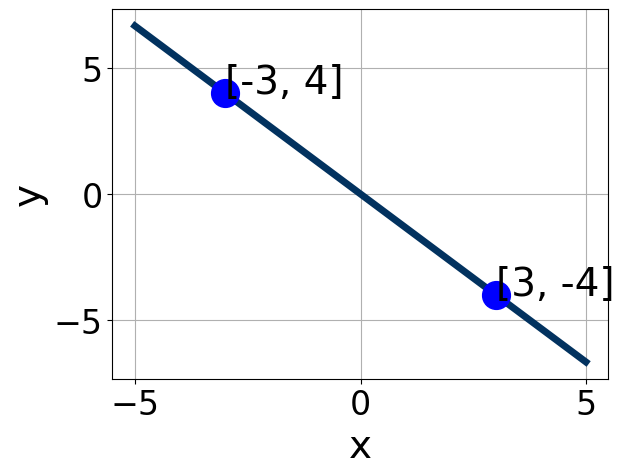
\includegraphics[width=0.5\textwidth]{../Figures/linearGraphToStandardC.png}
\end{center}
\begin{enumerate}[label=\Alph*.]
\item \( A \in [-5.1, -1.8], \hspace{3mm} B \in [-4.02, -2.14], \text{ and } \hspace{3mm} C \in [-6, 2] \)
\item \( A \in [-0.5, 2.4], \hspace{3mm} B \in [0.14, 2.7], \text{ and } \hspace{3mm} C \in [-6, 2] \)
\item \( A \in [2.8, 6.2], \hspace{3mm} B \in [-4.02, -2.14], \text{ and } \hspace{3mm} C \in [-6, 2] \)
\item \( A \in [-0.5, 2.4], \hspace{3mm} B \in [-1.95, 0.43], \text{ and } \hspace{3mm} C \in [-6, 2] \)
\item \( A \in [2.8, 6.2], \hspace{3mm} B \in [2.21, 3.98], \text{ and } \hspace{3mm} C \in [-6, 2] \)

\end{enumerate} }
\litem{
Solve the linear equation below. Then, choose the interval that contains the solution.\[ \frac{-5x -4}{7} - \frac{-3x + 8}{3} = \frac{6x -9}{8} \]\begin{enumerate}[label=\Alph*.]
\item \( x \in [-5.2, -3.2] \)
\item \( x \in [-1.7, 0.7] \)
\item \( x \in [-7.3, -5.8] \)
\item \( x \in [5.9, 7.5] \)
\item \( \text{There are no real solutions.} \)

\end{enumerate} }
\litem{
Solve the linear equation below. Then, choose the interval that contains the solution.\[ \frac{-5x + 3}{5} - \frac{-9x + 9}{7} = \frac{9x + 9}{8} \]\begin{enumerate}[label=\Alph*.]
\item \( x \in [-2.3, -0.9] \)
\item \( x \in [-18.2, -17.2] \)
\item \( x \in [0.4, 1.8] \)
\item \( x \in [-2, 0.1] \)
\item \( \text{There are no real solutions.} \)

\end{enumerate} }
\litem{
Write the equation of the line in the graph below in Standard Form $Ax+By=C$. Then, choose the intervals that contain $A, B, \text{ and } C$.
\begin{center}
    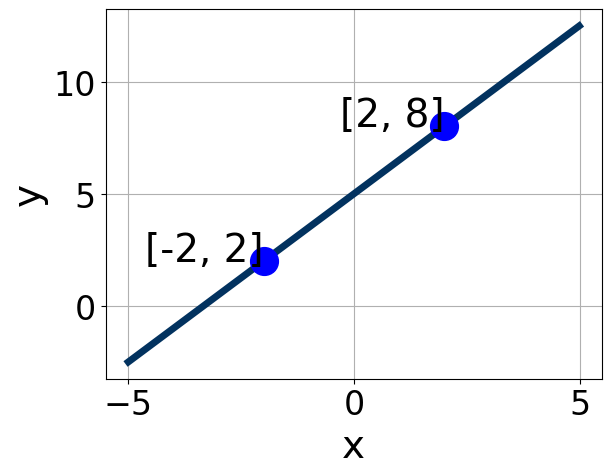
\includegraphics[width=0.5\textwidth]{../Figures/linearGraphToStandardCopyC.png}
\end{center}
\begin{enumerate}[label=\Alph*.]
\item \( A \in [-5.4, -2.4], \hspace{3mm} B \in [1.11, 3.02], \text{ and } \hspace{3mm} C \in [6, 11] \)
\item \( A \in [-2, -1.4], \hspace{3mm} B \in [-1.36, -0.52], \text{ and } \hspace{3mm} C \in [-6, -3] \)
\item \( A \in [-2, -1.4], \hspace{3mm} B \in [0.67, 1.45], \text{ and } \hspace{3mm} C \in [4, 7] \)
\item \( A \in [1.6, 5.1], \hspace{3mm} B \in [1.11, 3.02], \text{ and } \hspace{3mm} C \in [6, 11] \)
\item \( A \in [1.6, 5.1], \hspace{3mm} B \in [-2.35, -1.69], \text{ and } \hspace{3mm} C \in [-14, -7] \)

\end{enumerate} }
\litem{
Find the equation of the line described below. Write the linear equation in the form $ y=mx+b $ and choose the intervals that contain $m$ and $b$.\[ \text{Perpendicular to } 6 x - 5 y = 12 \text{ and passing through the point } (9, 5). \]\begin{enumerate}[label=\Alph*.]
\item \( m \in [-1.37, -1.11] \hspace*{3mm} b \in [11.5, 14.5] \)
\item \( m \in [0.34, 1.39] \hspace*{3mm} b \in [-3.5, -1.5] \)
\item \( m \in [-0.93, -0.78] \hspace*{3mm} b \in [-12.5, -11.5] \)
\item \( m \in [-0.93, -0.78] \hspace*{3mm} b \in [-5, -3] \)
\item \( m \in [-0.93, -0.78] \hspace*{3mm} b \in [11.5, 14.5] \)

\end{enumerate} }
\end{enumerate}

\end{document}